\usetikzlibrary{patterns}
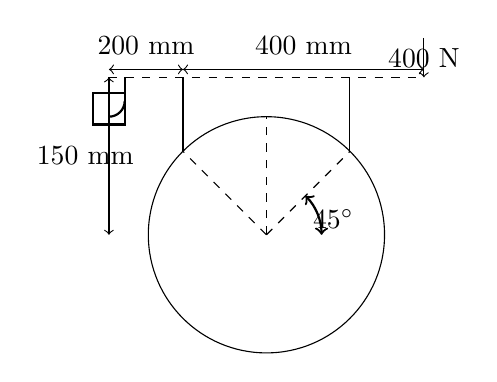
\begin{tikzpicture}
    % Drum
    \draw (0,0) circle (1.5cm); % Drum, assuming 300mm diameter scaled to 1.5cm in the diagram

    % Rod with arc and hinge
    \draw[thick] (-2, 2) -- (-2, 1.5); % Vertical part of the rod
    \draw[thick] (-2, 1.5) arc[start angle=270, end angle=360, radius=0.2cm]; % Small arc
    \draw[thick] (-1.8, 1.5) -- (-1.8, 2); % Connecting rod to hinge
    
    % Hinge (square) at the end of the rod
    \draw[thick] (-2.2, 1.4) rectangle (-1.8, 1.8); % Square hinge

    % Force
    \draw[->] (2, 2.5) -- (2, 2) node[above] {400 N}; % Force arrow with label

    % Dimensions and angle markings
    \draw[dashed] (0, 0) -- (0, 1.5); % Vertical reference from drum center
    \draw[dashed] (0, 0) -- (1.06, 1.06); % 45-degree line right
    \draw[dashed] (0, 0) -- (-1.06, 1.06); % 45-degree line left
    \draw (1.06, 1.06) -- (1.06, 2); % Line to top dimension
    \draw (-1.06, 1.06) -- (-1.06, 2); % Line to top dimension
    \draw[dashed] (-2, 2) -- (2, 2); % Top dashed line

    % 45 degree angle
    \draw[<->, thick] (0.7, 0) arc[start angle=0, end angle=45, radius=0.7cm];
    \node at (0.85, 0.2) {$45^\circ$}; % Angle label

    % Dimension labels
    \draw[<->] (-2.0, 2.1) -- (-1.06, 2.1) node[midway, yshift=0.3cm] {200 mm}; % 200 mm label
    \draw[<->] (-1.06, 2.1) -- (2, 2.1) node[midway, yshift=0.3cm] {400 mm}; % 400 mm label
    \draw[<->] (-2, 2) -- (-2, 0) node[midway, xshift=-0.3cm] {150 mm}; % 150 mm label
\end{tikzpicture}

